\documentclass[14pt]{amsart}
%\usepackage{amsmath}
\usepackage[utf8]{inputenc}
\usepackage{graphicx}
\usepackage{xcolor}
\usepackage[legalpaper, margin=1.0in]{geometry}
\usepackage{fancyvrb}
\usepackage{cprotect}
\usepackage{url}
\usepackage{etoolbox}
\usepackage{hyperref}
\usepackage[skins,theorems]{tcolorbox}
\usepackage{enumitem}
\newcommand*{\vertbar}{\rule[-1ex]{0.5pt}{2.5ex}}
\newcommand*{\horzbar}{\rule[.5ex]{2.5ex}{0.5pt}}
\setlist[itemize]{align=parleft,left=1pt..1em}

\usepackage{imakeidx}
\makeindex


\usepackage{cmbright}
\usepackage[OT1]{fontenc}


% fonts
%\input{ArtNouvc.fd}
%\newcommand*\initfamily{\usefont{U}{ArtNouvc}{xl}{n}}
%\usepackage[T1]{fontenc}
%\usepackage{tgbonum} % change font

%\usepackage[light,condensed,math]{iwona}
%\usepackage[T1]{fontenc}

% from https://www.pinterest.co.uk/pin/88664686405122253/
\definecolor{C1}{RGB}{141, 125, 158} %purple
\definecolor{C2}{RGB}{163,156,147} % yellow
\definecolor{C3}{RGB}{99,151,153} % green
\definecolor{C4}{RGB}{195,106,99} % red
\definecolor{C5}{RGB}{124, 132, 128}
\definecolor{C6}{RGB}{67, 69, 75}


\definecolor{Gr}{HTML}{377D71}
\definecolor{Pu}{HTML}{A459D1}
\definecolor{Bl}{HTML}{4D455D}
\definecolor{Te}{HTML}{C1ECE4}
\definecolor{Or}{HTML}{EF6262}
\definecolor{Am}{HTML}{F3AA60}
\definecolor{Co}{HTML}{3C486B}
\definecolor{Wh}{HTML}{FEFBF6}
\definecolor{Ye}{HTML}{FFE196}
\definecolor{Re}{HTML}{E96479}
\definecolor{Pi}{HTML}{FFD0D0}
\definecolor{Rp}{HTML}{FF9EAA}
\definecolor{Wg}{HTML}{EEF3D2}


\hypersetup{
    colorlinks=false,
    linkcolor=red,
    filecolor=red,      
    urlcolor=red,
    pdftitle={a},
    pdfpagemode=FullScreen,
    }
    
    
 % TCOLORBOX STUFF ----------------------------------------------------------------------------
 

 %  ----------------------------------------------------------------------------
    
\patchcmd{\section}{\normalfont}{\color{C5}}{}{}
\patchcmd{\subsection}{\normalfont}{\color{C5}}{}{}


\newcommand{\dfn}[1]{{\bf  \color{blue}{#1}}}


\renewcommand{\FancyVerbFormatLine}[1]{\color{gray}{>\,\,#1}}
    
\newtheorem{thm}{Theorem}


\newtheoremstyle{exercise}
{}                % Space above
{}                % Space below
{\color{black}}        % Theorem body font % (default is "\upshape")
{}                % Indent amount
{\bfseries}       % Theorem head font % (default is \mdseries)
{:}               % Punctuation after theorem head % default: no punctuation
{ }               % Space after theorem head
{}                % Theorem head spec
\theoremstyle{exercise}
\newtheorem{exercise}{Exercise}


\newtheoremstyle{example}
{}                % Space above
{}                % Space below
{\color{red}\slshape}        % Theorem body font % (default is "\upshape")
{}                % Indent amount
{\bfseries}       % Theorem head font % (default is \mdseries)
{.}               % Punctuation after theorem head % default: no punctuation
{ }               % Space after theorem head
{}                % Theorem head spec
\theoremstyle{example}
\newtheorem{example}{Example}

\newtheoremstyle{solution}
{}                % Space above
{}                % Space below
{\color{C5}}        % Theorem body font % (default is "\upshape")
{}                % Indent amount
{\bfseries }       % Theorem head font % (default is \mdseries)
{:}               % Punctuation after theorem head % default: no punctuation
{\newline}               % Space after theorem head
{}                % Theorem head spec
\theoremstyle{solution}
\newtheorem*{solution}{Solution}


\newcommand{\mcS}{\mathcal S}
\newcommand{\mcR}{\mathcal R}
\newcommand{\mcC}{\mathcal C}
\newcommand{\bS}{{\boldsymbol S}}
\newcommand{\bR}{{\boldsymbol R}}
\newcommand{\bC}{{\boldsymbol C}}
\newcommand{\ba}{{\boldsymbol a}}
\newcommand{\bb}{{\boldsymbol b}}
\newcommand{\bs}{{\boldsymbol s}}
\newcommand{\bff}{{\boldsymbol f}}
\newcommand{\br}{{\boldsymbol r}}
\newcommand{\bx}{{\boldsymbol x}}
\newcommand{\bt}{{\boldsymbol t}}
\newcommand{\bv}{{\boldsymbol v}}
\newcommand{\bu}{{\boldsymbol u}}
\newcommand{\bw}{{\boldsymbol w}}
\newcommand{\bc}{{\boldsymbol c}}
\newcommand{\be}{{\boldsymbol e}}
\newcommand{\bq}{{\boldsymbol q}}
\newcommand{\bphi}{{\boldsymbol \phi}}
\newcommand{\brho}{{\boldsymbol \rho}}
\newcommand{\btau}{{\boldsymbol \tau}}
\newcommand{\reals}{\mathbb R}
\newcommand{\ints}{\mathbb N}
\newcommand{\E}{\mathbb E}
\newcommand{\Prob}{\mathbb P}


%%%%%%%%%%%%%%%




\begin{document}



\title{Regression with multiple predictors}
\maketitle
%----------------------------------------------------------------------------------------------------------------
\section{Reading}
\begin{itemize}
\item  \cite[Section 10.1]{islp}
\begin{itemize}
\item Example 10.1.2. This is the linear regression model with multiple predictors. 
\item This entire section is useful and all the exercises are good practice. 
\end{itemize}
\item \cite[Section 10.2]{tabak}
\item \cite[Section 10.5]{tabak}
\item \cite[Section 3.2]{islp}
\end{itemize}

%----------------------------------------------------------------------------------------------------------------
\section{Learning objectives}

\begin{itemize}
\item Understand how to simulate and fit linear regression models with multiple predictors. 
\item Interpret regression coefficients in linear regression with multiple predictors. 
\end{itemize}


\section{Multiple predictor linear regression}
\begin{itemize}
\item The real power of regression comes when we work with models of the form 
\begin{align}
Y &= \beta_0 + \sum_{i=1}^K \beta_iX_i + \epsilon\\
\epsilon &\sim {\rm Normal}(0,\sigma^2)
\end{align}
where $X_i$ is a set of $K$ predictor variables. Alternatively, we can write
\begin{equation}
Y|(X_1=x_1,\dots,X_K=x_K) \sim {\rm Normal}\left( \beta_0 + \sum_{i=1}^K \beta_iX_i,\sigma^2\right)
\end{equation}
I will also use the shorthand, 
\begin{equation}
Y \sim {\rm LR}(X,\beta,\sigma^2). 
\end{equation}
I will also use the notation 
\begin{equation*}
\hat{y} = \hat{\beta}_0 + \sum_{i=1}^K \hat{\beta}_iX_i 
\end{equation*}
to refer to the predicted value of $E[Y|X]$ after fitting a regression model. 

In these notes, our goal is to answer the following questions
\begin{enumerate}
\item What are estimators of the parameters in this model?
\item How do we interpret the \dfn{regression coefficients} $\beta_i$? 
\item Precisely what are the assumptions we are making when we use a linear regression model? 
\item How do we access the model assumptions? 
\end{enumerate}



%\subsection{Multiple predictors in python}
\begin{example}[Simulating and fitting a regression with two predictors]
See \href{https://colab.research.google.com/drive/1oIRgP_7-c5DGV1D2iz5nj406mZfJxUIG?usp=sharing}{colab notebook}. 
\end{example}

\item The output from the regression with multiple predictors is basically the same as for single-predictor, except now we have multiple rows for the difference regression coefficients. In each case, the interpretation of the $p$-value and confidence intervals are nearly the same as they were for the single predictor case. However, for the $p$-value, we need to remember that this is the $p$-value testing the hypothesis that a particular predictor is zero. The $F$-statistic is used to test the hypothesis that all predictors are zero, although I won't go into much more detail because I don't place a big emphasis on hypothesis testing in this course. 

\item The interpretation of $R^2$ is the same as before, except that now we are considering the ratio of the variance conditioned on ALL predictors to the overall variation in $Y$; that is, 
\begin{equation*}
R^2 = 1 - \frac{\sum_i r_i^2}{\sum_i (y_i - \bar{y})^2}    \approx 1 - \frac{{\rm var}(Y|X_1,X_2)}{{\rm var}(Y)}
\end{equation*} 
where in the multi-predictor case 
\begin{equation}
r_i = Y_i - \left(\hat{\beta}_0 + \sum_k^m \hat{\beta}_kX_{i,k}\right). 
\end{equation} 

\end{itemize}

%\begin{example}
%\href{}{Our first regression with multiple predictors}
%\end{example}


\begin{figure}[h!]
    \centering
    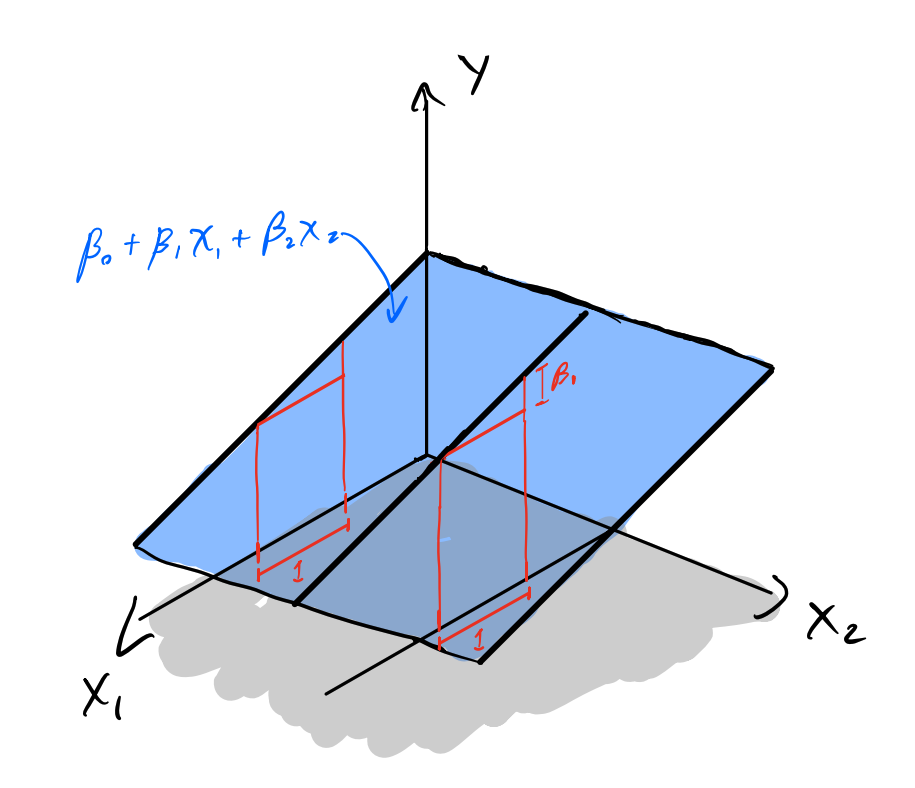
\includegraphics[width=0.8\textwidth]{./../figures/plane}
    \caption{The function $y(x_1,x_2)$}
    \label{fig:plane}
\end{figure}

\subsection{Basic interpretation and estimation of the parameters }
\begin{itemize}
\item In order to interpret the parameters, it's easiest to work with just two predictors like we have in the example above. The formula for the conditional expectation of $Y$ is 
\begin{equation}\label{eq:2dsurface}
E[Y|X] = \beta_0 + \beta_1X_1 + \beta_2X_2
\end{equation}
where I'm using the shorthand 
\begin{equation*}
E[Y|X] = E[Y|(X_1,X_2)]
\end{equation*}
to mean the expected value of $Y$ conditioned on both predictors. 



Equation \ref{eq:2dsurface} is the equation for a flat surface in two dimensions: 
\begin{equation}
y = \beta_0 + \beta_1x_1 + \beta_2x_2
\end{equation}
A drawing of $y$ is shown in \ref{fig:plane}. 


 \item If we make a slice through the surface in the $x_1$ direction and look it at from the side, we see a line with slope $\beta_1$ (and similarly for $x_2$).  This leads to the following interpretation of $\beta_i$:  
 \begin{center}
 $\beta_1$ is the slope of $E[Y|X]$ vs. $X_1$ for fixed $X_2$. 
 \end{center}
Notice that in the statement above, even though we are conditioning on both variables, the slope $\beta_1$ is independent of which value of $X_2$ we condition on. We can obtain the interpretation of $\beta_2$ by flipping the role of $X_1$ and $X_2$. 
The fact that is doesn't matter which value of $X_2$ (respectively $X_1$) we have conditioned on is one of the core model assumption of linear regression with multiple predictors, which we do not encounter in the single predictor case. Another way of articulating it is to say: the ``effect'' of $X_1$ and $X_2$ are not dependent on the other predictors value.
\item In the case of children's test scores, we are saying that the association between the mother's high school education and test scores is not influenced by the mother's IQ. that is, If we compare two random children whose mothers have the same IQ, differ in whether they attended high school, then the average \emph{difference} between their test scores will not depend on the IQ of their mothers, although the average magnitude of their test scores will depend on the mother's IQ. 



\begin{example}[Test scores]
Consider the example of children's test scores, but now we will have two predictors: $X_{\rm iq}$ representing the mother iq and $X_{\rm hs}$ representing whether the mother went to high school. \\


\noindent
\underline{Question:} Fit the data to a linear regression model with two predictors and answer the questions
\begin{enumerate}[label=(\alph*)]
\item What are the regression coefficients and the interpretations? 
\item Based on this regression analysis, which factor, IQ or high school education do we believe is more predictive of test scores? 
\item Overall, how well do high school education and IQ os methods do at predicting the test scores of children? 
\item What is the chance a student whose mother has an IQ of $90$ and did not go to high school does better than a student whose mother has an IQ of $110$ and did go to high school?\\
\end{enumerate}



\noindent
\underline{Solutions:}
We get the following output from \verb!statsmodels! in the \href{https://colab.research.google.com/drive/1oIRgP_7-c5DGV1D2iz5nj406mZfJxUIG?usp=sharing}{colab notebook}:\\

\noindent
\begin{Verbatim}
                            OLS Regression Results                            
==============================================================================
Dep. Variable:                      y   R-squared:                       0.214                                   
==============================================================================
                 coef    std err          t      P>|t|      [0.025      0.975]
------------------------------------------------------------------------------
const         25.7315      5.875      4.380      0.000      14.184      37.279
mom_hs         5.9501      2.212      2.690      0.007       1.603      10.297
mom_iq         0.5639      0.061      9.309      0.000       0.445       0.683


\end{Verbatim}
\vspace{1cm}
\begin{enumerate}[label=(\alph*)]
\item For the regression coefficients we find the follow:
\begin{itemize}
\item $\beta_{\rm hs} \approx 5.95$. This means that among students whose mothers {\bf have the same IQ}, a student whose mother attended high school will, on average, have a score that is $5.95$ points higher than a student whose mother did not. 
\item $\beta_{\rm iq} \approx 0.56$. This means that among students whose mother's {\bf have the same high school education} (either they all attended or did not attend high school), the difference between scores of students whose mothers IQ differs by one point is, on average, $0.56$ points.
\item $\hat{\beta}_0 \approx 26$. Mathematically, this tells us the average score of students whose mother did not attend high school and have zero IQ, but this is not a meaningful quantity since noone has zero iq. We can therefore ignore it when it comes to interpreting the output. 
\end{itemize}
\item Clearly $\beta_{\rm hs}$ is smaller, but we need to remember that are comparing quantities that have different units. $X_{\rm iq}$ takes values from around 70 to 130, while $X_{\rm hq}$ is either zero or 1. What is actually more useful is to compare how much a difference in one standard deviation of the predictor makes. For example, $\beta_{\rm iq}\sigma_{\rm iq}$ is the average difference in test scores between students whose mothers have the same high school education, but whose mother's IQ differ by one standard deviation. To this end, we can compute the following measures of effects
\begin{align*}
\hat{\beta}_{\rm hs}\hat{\sigma}_{\rm hs} &\approx 2.44\\
\hat{\beta}_{\rm iq}\hat{\sigma}_{\rm iq} &\approx 8.44.
\end{align*}
The association between IQ and scores is actually larger. Note that the comparison is not perfect, since $X_{\rm hs}$ is a binary variable, but it still gives us a generally idea of the effects. \\
\item The $R^2$ value is $0.214$, so about $20\%$ of the variation in test scores is explained by the variation in high school education and IQ of mothers. 
\item In the colab notebook we calculate this to be about $25\%$. 
\end{enumerate}
%
%Let's start by seeing how to work with multiple predictors in python
%The first step is to get the predictor variables in the correct format for statsmodels. Statsmodels wants us to input a multidimensional arrray 
%\begin{equation}
%X = \left[\begin{array}{ccc}
%1 &x_{1,1}& x_{1,2}\\
%1 &x_{2,1}& x_{2,2}\\
%\vdots & \vdots & \vdots\\
%1 &x_{n,1}& x_{n,2}\\
%\end{array} \right]
%\end{equation}
%
%The $i$th column contains the predictors that go with our $i$th observation $y$. This will tell statsmodels to also include a constant term (the intercept) $\beta_0$ in our regression. 
%
%The following code will get our data in this format:
%\begin{Verbatim}
%X = sm.add_constant(np.transpose(np.array([x_hs,x_iq])))
%\end{Verbatim}
%%\href{https://colab.research.google.com/drive/1oIRgP_7-c5DGV1D2iz5nj406mZfJxUIG#scrollTo=wbeO1TS8os5J&line=15&uniqifier=1}{Our first regression with multiple predictors}
\end{example}
\end{itemize}

\subsection{Interpretation of regression coefficient: a deeper look}
\begin{itemize}

\item   We can express the regression coefficients explicitly in terms of conditional averages as
 \begin{equation}\label{eq:beta1exp}
 \beta_1 = E[Y|X_1 = (x+1),X_2] -  E[Y|X_1 = x,X_2].
 \end{equation}
Now let's think about how the regression coefficients are related to covariance. One guess would be that, just as in the single-predictor case, $\beta_1$ is given by ${\rm cov}(Y,X_1)/\sigma_{x_1}^2$. After all, if we look a slice of the 2D planer function $y(x_1,x_2)$ along the $x_1$ direction, we get the same slope for all $x_2$.  It stands to reason that if we look at only the points in the $x_1$-$y$ plane our regression slope would be $\beta_1$. However, {\bf this argument assumes that when we change $x_1$, $x_2$ does not also change}. This is best understood with an example. 


\begin{example}[Test scores with multiple vs. single predictors]
Here we will consider once again the example of children's test scores and compare using both predictors in the sample above to the results we obtain we using only one predictor (high school education). \\



\noindent
\underline{Question:} What is the difference between the coefficient of $X_{\rm hs}$ when this is the only predictor and the coefficient when $X_{\rm iq}$ is also used? How is the coefficient in the multiple predictor case related to coefficient in the single predictor case?  \\

\noindent
\underline{Solution:} When we performed the regression using only the mother's high school education as a predictor, we obtained a coefficients of about $\hat{\beta}_{\rm hs}' \approx 12$ and $\hat{\beta}_0' \approx 78$ (i'll use $\beta'$ indicate coefficients in the single predictor model, as opposed to the multiple predictor model). The fitted model is
\begin{equation*}
\hat{y} = 12X_{\rm hs} + 78 
\end{equation*}
while when also using $X_{\rm iq}$ as a predictor,  the coefficient is about half that.


In the model with one predictor, the regression coefficient of $12$ means that on average a student whose mother went to high school will do $12$ points better than one whose mother did not.  That is, we are predicting
\begin{equation*}
E[Y|X_{\rm hs} = 1]-E[Y|X_{\rm hs} = 0]  = \beta_{\rm hs}' \approx 12
\end{equation*}
Let's compare this to what we would predict in the model with two predictors. 
In that case, the average test score of student whose mother went to high school is
\begin{align*}
\hat{y}_{\rm hs} &\approx E[Y|X_{\rm hs} =1]\\
&=  E[\beta_0 +  \beta_{\rm hs} +\beta_{\rm iq}X_{\rm iq} |X_{\rm hs}=1]\\
&=\beta_0 +  \beta_{\rm hs} +\beta_{\rm iq}E[X_{\rm iq}|X_{\rm hs}=1]\\
&\approx  6\times 1+ 26  +  0.6 \overline{X}_{{\rm iq}|{\rm hs}} 
\end{align*}
where 
\begin{equation*}
\overline{X}_{{\rm iq}|{\rm hs}}  =  \text{sample average IQ of mother who attended high school} \approx E[X_{\rm iq}|X_{\rm hs}=1]
\end{equation*}

On the other hand 
\begin{equation*}
\hat{y}_{\rm no-hs} =  6 \times 0 + 26  +  0.6 \overline{X}_{{\rm iq},{\rm no-hs}} 
\end{equation*}
where 
\begin{equation*}
\overline{X}_{{\rm iq}|{\rm no-hs}}  = \text{sample average IQ of mother who DID NOT attend high school} \approx  E[X_{\rm iq}|X_{\rm hs}=0]
\end{equation*}


Thus, according to the model with two predictors, the average difference in test scores between the \verb!hs! and \verb!no-hs! groups is 
\begin{equation*}
\Delta \hat{y}_{\rm hs} = 6 +0.6(\overline{X}_{{\rm iq}|{\rm hs}}-\overline{X}_{{\rm iq}|{\rm no-hs}} )
\end{equation*}
or written in terms of more probabilistic notation 
\begin{equation*}
E[Y|X_{\rm hs} = 1]-E[Y|X_{\rm hs} = 0]  = \beta_{\rm hs} + \beta_{\rm iq}(E[X_{\rm iq}|X_{\rm hs} = 1]-E[X_{\rm iq}|X_{\rm hs} = 0]  )
\end{equation*}
We can compute $\overline{X}_{{\rm iq}|{\rm hs}}-\overline{X}_{{\rm iq}|{\rm no-hs}} \approx 10.3$, which gives $\Delta \hat{y}_{\rm hs} \approx 12$. Thus, we have calculated the single-predictor regression coefficient from the multiple predictor case.  





\end{example}




  
%  \begin{example}
%\href{https://colab.research.google.com/drive/1oIRgP_7-c5DGV1D2iz5nj406mZfJxUIG#scrollTo=wbeO1TS8os5J&line=15&uniqifier=1}{Understanding the multiple predictors regression slopes}
%\end{example}
  
\item The important thing is that the two predictors are in independent. If they were, then $\overline{X}_{{\rm iq}|{\rm hs}}-\overline{X}_{{\rm iq}|{\rm no-hs}}$ would be zero, and it would have to be that the coefficient of $X_{\rm hs}$ is the same in both cases. We can generalize this to any model where $X_1$ is a binary predictor to obtain a relationship between the regression coefficient for $\beta_1$ with and without the second predictor; that is, 
\begin{equation*}
\beta_1' = \beta_1 + \beta_2(E[X_2|X_1=1]-E[X_2|X_1=0])
\end{equation*}
where $\beta_1'$ is the regression coefficient without using $X_2$ as a predictor in our model. 
\item Now we will dig deeper into the underlying, math, with the goal of better understanding how the relationship between predictors shapes the regression coefficients. A byproduct of this exploration will be formulas for the regression coefficients in terms of covariances between the predictors, and covariance between the predictors and the response variable. These formulas generalize the relationship ${\rm cov}(X,Y) = \beta_1\sigma_x^2$, which we discovered to hold in the single predictors case. 


\begin{figure}[h]
    \centering
    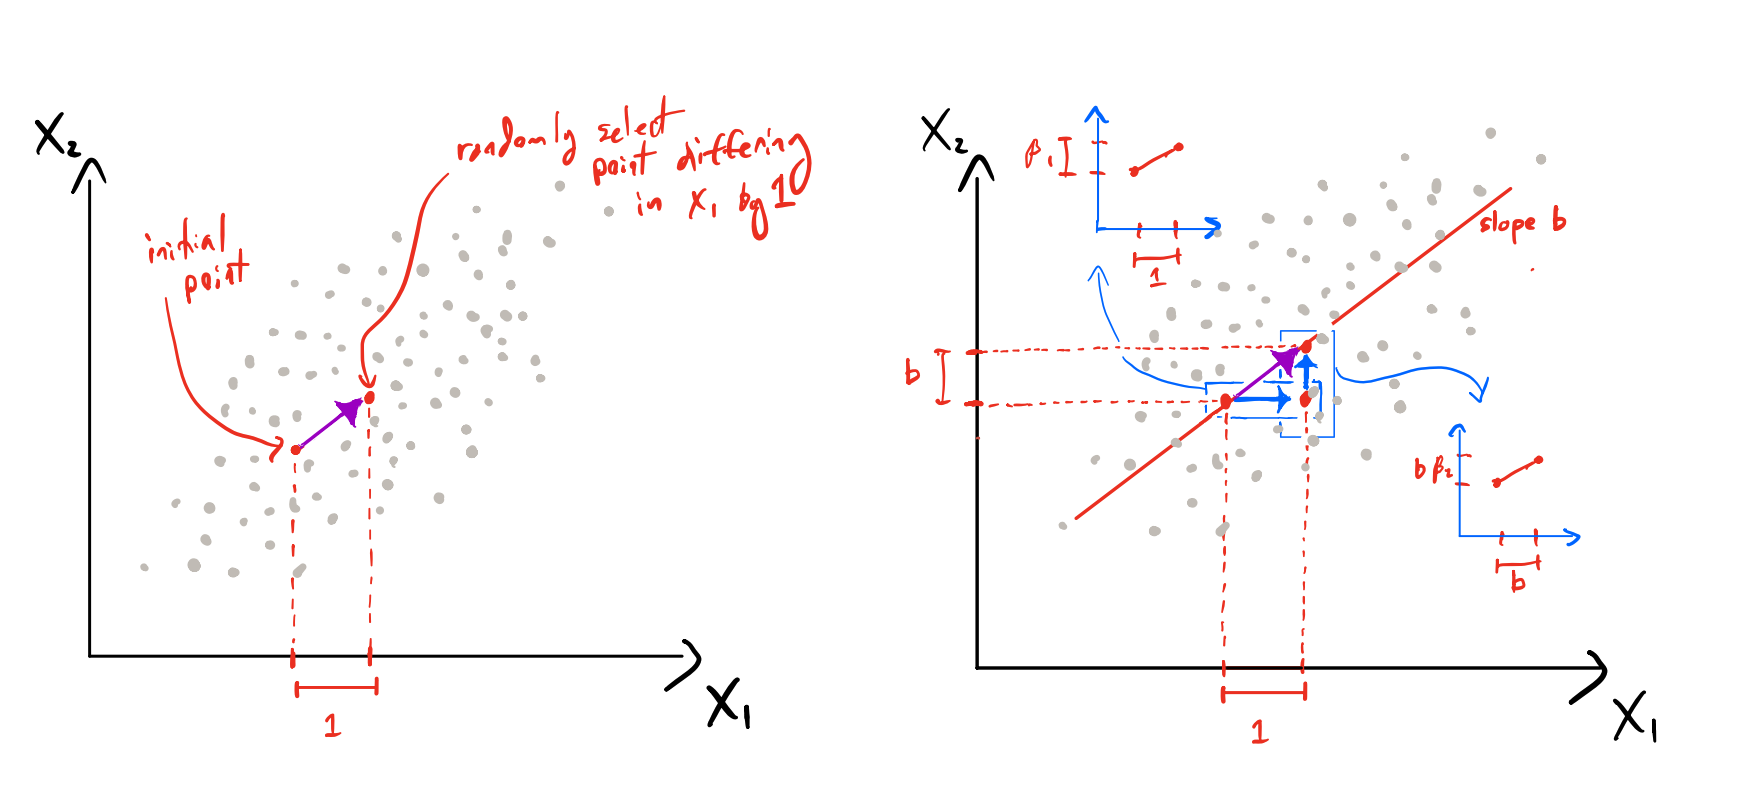
\includegraphics[width=0.8\textwidth]{./../figures/correlated_predictors}
    \caption{Here I'm illustrated the difference between the marginal regression slope (the slope of $E[Y|X_1]$ vs. $X_1$) and the regression coefficient $\beta_1$ in the two predictor model.  I use the notation of Example \ref{ex:normal_pred}, although the idea applies more generally. When we increase $x_1$ by $1$ without fixing $X_2$, then on average $X_2$ changes by $b$ (which is the slope between $x_1$ and $x_2$ here, not the intercept.) Therefore, in order to relate this marginal slope to the regression slooe $\beta_1$, subtract the increase in $Y$ that is caused by the increase in $X_2$ (corresponding to the vertical blue arrow).   }
    \label{fig:plane}
\end{figure}

\item Consider a generic linear regression model with two predictors. We will set $\beta_0=E[X_1]=E[X_2]=0$ for simplicity, since these cancels out in the end. We start by computing ${\rm cov}(X_1,Y)$, which is simply $E[X_1Y]$ since $E[X_1]=E[Y] = 0$. 
%\begin{equation*}
%E[Y] = \beta_0 + \beta_1E[X_1]+\beta_2E[X_2]=0. 
%\end{equation*}
Just as we did for the single-predictor case (week 3), we write
\begin{align*}
{\rm cov}(X_1,Y) &= E[X_1Y] = E[X_1E[Y|X_1]] \\
&= E[X_1(\beta_1 X_1 + \beta_2 X_2)] = \beta_1 E[X_1^2] + \beta_2 E[X_1X_2]\\
&= \beta_1 \sigma_{x_1}^2  + \beta_2 {\rm cov}(X_1,X_2)
\end{align*}
where we have used that, since $E[X_1]=E[X_2]=0$, ${\rm var}(X_1) = E[X_1^2]$ and ${\rm cov}(X_1,X_2) = E[X_1X_2]$.
 If we do the same for $X_2$, we get two equations
 \begin{align*}
 {\rm cov}(X_1,Y)  &= \beta_1 \sigma_{x_1}^2  + \beta_2 {\rm cov}(X_1,X_2)\\
{\rm cov}(X_2,Y) &=   \beta_2 \sigma_{x_2}^2  + \beta_1 {\rm cov}(X_1,X_2)
 \end{align*}
As with the single-predictor case, it is very useful to represent $\beta_1$ and $\beta_2$ as expectations which can be computed as averages over our data points. In addition to providing some insight into the meaning of the regression coefficients, this will yield candidates for our estimators of these quantities. 
Since everything in the equation can be represented as a some sort of expectation except the coefficients $\beta_1$ and $\beta_2$, we just need to solve for these coefficients. Solving the linear system  
\begin{align*}
\left[\begin{array}{c}
{\rm cov}(X_1,Y) \\
{\rm cov}(X_2,Y)  
\end{array}\right] &= \left[\begin{array}{cc}
\sigma_{x_1}^2 & {\rm cov}(X_1,X_2)\\
 {\rm cov}(X_1,X_2) & \sigma_{x_2}^2
 \end{array} \right]\left[ \begin{array}{c}
\beta_1\\
  \beta_2\\
  \end{array}\right]
\end{align*}
yields 
\begin{align*}
\left[\begin{array}{c}
\beta_1 \\
\beta_2 
\end{array}\right] &= \left[\begin{array}{cc}
\sigma_{x_1}^2 & {\rm cov}(X_1,X_2)\\
 {\rm cov}(X_1,X_2) & \sigma_{x_2}^2
 \end{array} \right]^{-1}\left[ \begin{array}{c}
 {\rm cov}(X_1,Y)\\
  {\rm cov}(X_2,Y)\\
  \end{array}\right]\\
  &=  \frac{1}{\sigma_{x_2}^2\sigma_{x_1}^2 -{\rm cov}(X_1,X_2)^2} \left[\begin{array}{cc}
\sigma_{x_2}^2 & -{\rm cov}(X_1,X_2)\\
- {\rm cov}(X_1,X_2) & \sigma_{x_1}^2
 \end{array} \right]\left[ \begin{array}{c}
 {\rm cov}(X_1,Y)\\
  {\rm cov}(X_2,Y)\\
  \end{array}\right]
%  &=\left[\begin{array}{c}
%   \frac{ {\rm cov}(X_1,Y)\sigma_{x_2}^2 - {\rm cov}(X_2,Y){\rm cov}(X_1,X_2)}{\sigma_{x_2}^2\sigma_{x_1}^2 -{\rm cov}(X_1,X_2)^2}\\
%     \frac{ {\rm cov}(X_2,Y)\sigma_{x_1}^2 - {\rm cov}(X_1,Y){\rm cov}(X_1,X_2)}{\sigma_{x_2}^2\sigma_{x_1}^2 -{\rm cov}(X_1,X_2)^2}
%  \end{array}
%  \right]
\end{align*}
After using the formula for the inverse of $2\times 2$ matrix, we obtain 
\begin{align}\label{eq:beta1cov}
\beta_1 =     \frac{ {\rm cov}(X_1,Y)\sigma_{x_2}^2 - {\rm cov}(X_2,Y){\rm cov}(X_1,X_2)}{\sigma_{x_2}^2\sigma_{x_1}^2 -{\rm cov}(X_1,X_2)^2}
%&= \frac{ {\rm cov}(X_1,Y)- {\rm cov}(X_2,Y){\rm cov}(X_1,X_2)/\sigma_{x_2}^2 }{\sigma_{x_1}^2 -{\rm cov}(X_1,X_2)^2/\sigma_{x_2}^2 }
\end{align}
%We can rewrite this as
%\begin{align*}
%\beta_1 =    \frac{ {\rm cov}(X_1,Y)\sigma_{x_2}^2 - {\rm cov}(X_2,Y){\rm cov}(X_1,X_2)}{\sigma_{x_2}^2\sigma_{x_1}^2 -{\rm cov}(X_1,X_2)^2}
%\end{align*}\

The formula is particularly revealing if all the variances are set to one\textcolor{orange}{
\begin{equation*}
\beta_1 = \frac{1}{1-\rho_{1,2}^2}(\rho_1 - \rho_{1,2}\rho_2)
\end{equation*}}
where $\rho_{1,2}$ is the correlation coefficient between $X_1$ and $X_2$. Notice that if $X_1$ and $X_2$ are uncorrelated ($\rho_{1,2}=0$), we obtain the usual connection between the regression coefficient and the correlation coefficient between $X_1$ and $X_2$. 
%
%
%This is not the same as the regression slope of $Y$ vs. $X_1$. Why? 
%\begin{align}
%\tilde{a}_1 &= \E[Y|X_1=(x+1)] -  \E[Y|X_1=x] \\
%&= a_1+ \underbrace{a_2( \E[X_2|X_1=(x+1)]- \E[X_2|X_1=x])}_{=\delta_{1,2}}
%\end{align}
%The second contribution $\delta_{1,2}$ characterizes the change in slope as a result of a bias towards higher or lower values of $x$. Notice that, if we were to model for $X_2$ vs $X_2$ with slope $u$, then 
%\begin{equation}
%\delta_{1,2} = a_2u
%\end{equation}
%We can understand this geometrically if we visualize the $X_2$ vs. $X_1$ plain from above. 
%
\begin{example}[Correlated predictors]\label{ex:normal_pred}
Consider the model
\begin{align*}
X_1 &\sim {\rm Normal}(0,1)\\
X_2|X_1 &\sim {\rm Normal}(bX_1,1-b^2)\\
Y|(X_1,X_2) & \sim {\rm Normal}(\beta_1X_1 + \beta_2X_2,\sigma^2). 
\end{align*}


\noindent
\underline{Question:} 
\begin{enumerate}[label=(\alph*)]
\item Show that ${\rm var}(X_1) = {\rm var}(X_2) = 1$ and ${\rm cov}(X_1,X_2)=b$
\item Expression $\beta_1$ as a function of $b$. 
\item Test Equation \ref{eq:beta1cov} with simulations. \\
\end{enumerate}



\noindent
\underline{Solution:} 
\begin{enumerate}[label=(\alph*)]
\item By definition of the model ${\rm var}(X_1)=1$ and 
\begin{align*}
{\rm var}(X_2) &= b^2{\rm var}(X_1) + 1-b^2 = b^2+1-b^2 = 1\\
{\rm cov}(X_1,X_2) &= b{\rm var}(X_1) = b
\end{align*}
\item We can write Equation \ref{eq:beta1cov} as
\begin{equation*}
\beta_1 =  \frac{ {\rm cov}(X_1,Y)- {\rm cov}(X_2,Y)b}{1 -b^2}
\end{equation*}
\item See \href{https://colab.research.google.com/drive/1oIRgP_7-c5DGV1D2iz5nj406mZfJxUIG?usp=sharing}{colab notebook}.
\end{enumerate}

%\noindent
%\underline{Solution:} In order to apply Equation \ref{eq:beta1cov}, we need to determine $\sigma_{x_1}$, $\sigma_{x_2}$ and the covariances. In the notation of the problem $\sigma_{x_1} = \sigma_1$ and setting $\sigma_2 = \sigma_{x_2}$, we have
%\begin{align*}
%\sigma_{2}^2 &=  b^2\sigma_{1}^2 + \sigma_{2|1}^2\\
%{\rm cov}(X_1,X_2) &= b\sigma_1\\
%{\rm cov}(X_1,Y) &= 
%\end{align*}

\end{example}

\item This can all be generalized to the situation where we have many predictors. The general formula for the regression coefficient in terms of expectation is 
\begin{align*}
\begin{split}
\beta_i &= E[Y|X_1,\dots,X_{i-1},X_i=x_i+1,X_{i+1},\dots,X_K]\\
&\quad\quad - E[Y|X_1,\dots,X_{i-1},X_i=x_i,X_{i+1},\dots,X_K]
\end{split}
\end{align*}
Note how this is a very natural extension of Equation \ref{eq:beta1exp}. 
We get a more complex expression for the coefficients but the idea is the same. 

\end{itemize}

\section{Collinearity and sloppiness}
\begin{itemize}
\item {\bf The sample distribution of coefficients}
Just as before, we want to understand what the sample distribution of the coefficients looks like. In the multiple predictor case, we need to think about the joint distribution  of $(\hat{\beta}_1,\hat{\beta}_2,\dots,\hat{\beta}_M)$. We will start by focusing on the two predictor case.  



\begin{figure}[h]
    \centering
    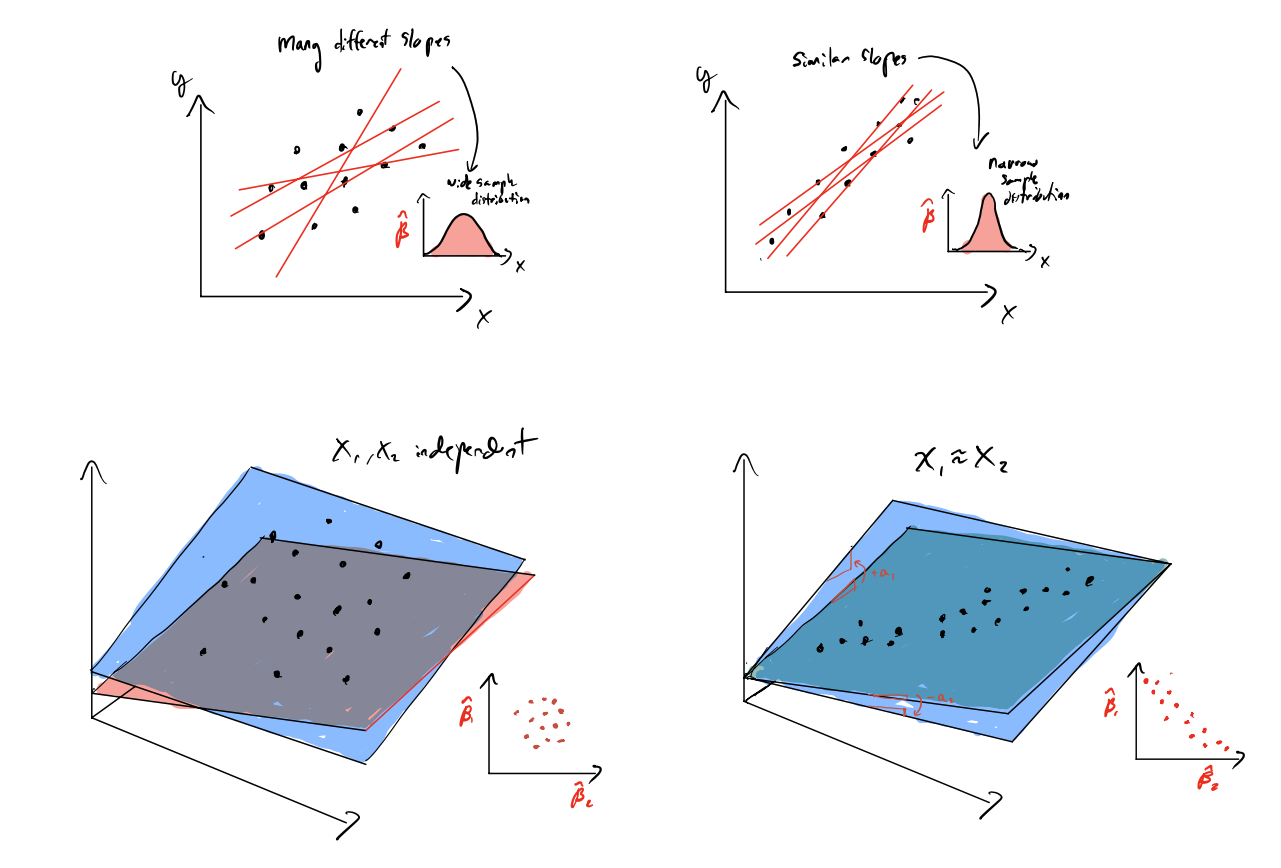
\includegraphics[width=0.8\textwidth]{./../figures/sample_dist}
    \caption{(top) In the single-predictor case, the width of the sample distribution measures how confident we are of a particular slope. It will be narrow if a replicate of our data is likely to produce a very similar slope.  These means we get a rough idea of the width of sample distribution by seeing much we can change our regression line and still obtain something that appears to pass through our data. (bottom) In the two predictor case, we have a regression plane and changing $\beta_1$ and $\beta_2$ will ``wiggle" the plane by tilting it in the $x_1$ and $x_2$ directions (there is also the intercept which can shift the plane up and down, but I'm not illustrating that). If $X_1$ and $X_2$ are uncorrelated, it doesn't matter which way we wiggle it, the fit will be similar, but if $X_1$ and $X_2$ are strongly correlated, wiggling the plane in the direction perpendicular  to the points has a much smaller effect that parallel to them. }
    \label{fig:sample_dist}
\end{figure}



%\begin{example}
%\href{https://colab.research.google.com/drive/1oIRgP_7-c5DGV1D2iz5nj406mZfJxUIG#scrollTo=h_vbLZqWPNzD&line=1&uniqifier=1}{Understanding multivariate sample distribution}
%\end{example}
\begin{example}[Predictor sample distribution]

Consider the model in \ref{ex:normal_pred}. Let's look at the sample distribution by fitting many simulated replicates. \\

\noindent
\underline{Question:} Write a function to generate a dataframe containing samples from the sample distribution of $(\hat{\beta}_1,\hat{\beta}_2)$. Make a scatter plot and explore the structure of the sample distribution, in particular it dependence on $b$, which controls the correlations between $X_1$ and $X_2$. \\


\noindent
\underline{Solution:} 
See \href{https://colab.research.google.com/drive/1oIRgP_7-c5DGV1D2iz5nj406mZfJxUIG?usp=sharing}{colab notebook}

\end{example}

To better understand what is going on, imagine $X_1$ and $X_2$ are very highly correlated (if they are perfectly correlated we say they are \dfn {colinear}). We can then write 
\begin{align*}
Y &= \beta_1X_1 + \beta_2X_2 + \epsilon  \approx \beta_1X_1 + \beta_2X_1 + \epsilon\\
 &\approx (\beta_1+\beta_2)X_1 + \epsilon
\end{align*}
There are many ways to select $\beta_1$ and $\beta_2$ so that the surface $\beta_1x_1+a_2\beta_2$ is close to the lines, since a change in $\beta_1$ can be compensated by a change in $\beta_2$. This means that {\bf if we estimate $\beta_1$ and $\beta_2$ and then generated new data, it would be possible to get a VERY different value of $\hat{\beta}_1$ and $\hat{\beta}_2$, so long as $\hat{\beta}_1 + \hat{\beta}_2$ is close to what we got before}. This is illustrated in Figure \ref{fig:sample_dist} and Figure \ref{fig:sample_dist2}. 

\begin{figure}[h]
    \centering
    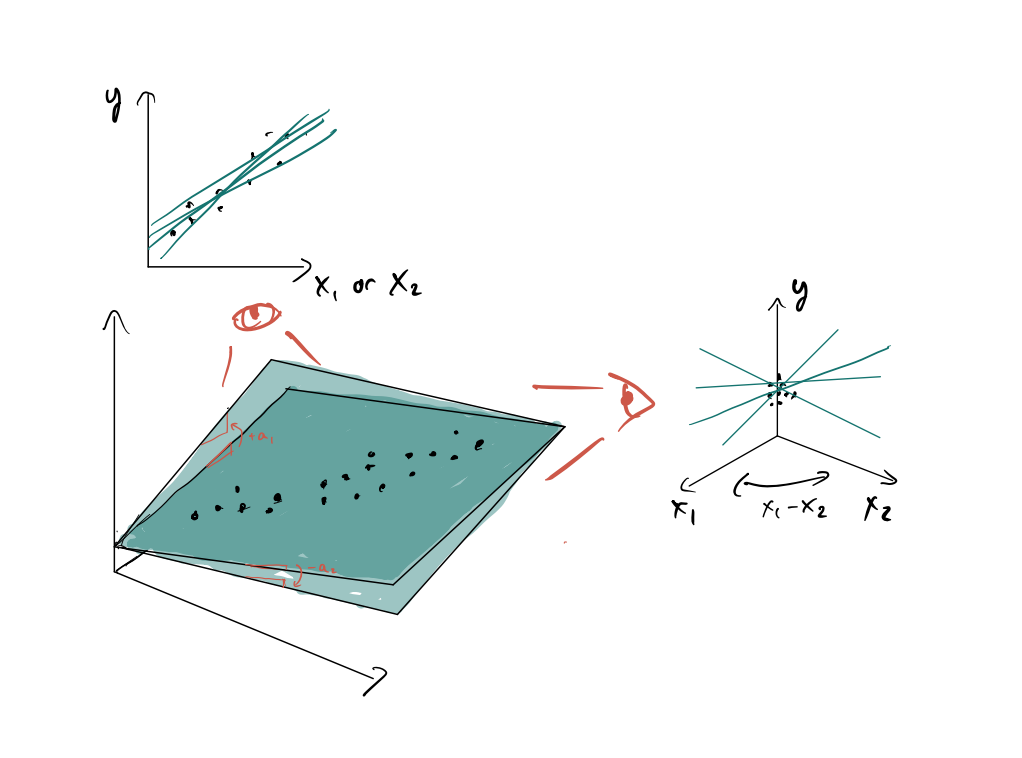
\includegraphics[width=0.8\textwidth]{./../figures/sample_dist2}
    \caption{Different views of the data in the case when $X_1$ and $X_2$ are correlated. If we look at the data from the side, or along the $X_1=X_2$ direction, then all our regression planes appear similar; however, when looked at from the ``front" as shown in the right panel, we see that the places actually have very different slopes in the other direction.  }
    \label{fig:sample_dist2}
\end{figure}




%\begin{exercise}
%\href{https://colab.research.google.com/drive/1oIRgP_7-c5DGV1D2iz5nj406mZfJxUIG#scrollTo=h_vbLZqWPNzD&line=1&uniqifier=1}{Understanding multivariate sample distribution}
%\end{exercise}
%
%\begin{exercise}
%\href{https://colab.research.google.com/drive/1oIRgP_7-c5DGV1D2iz5nj406mZfJxUIG#scrollTo=SugKDnavWgtU&line=3&uniqifier=1}{Sample distributions and predictors}
%\end{exercise}
%
%\begin{exercise}
%\href{https://colab.research.google.com/drive/1oIRgP_7-c5DGV1D2iz5nj406mZfJxUIG#scrollTo=SugKDnavWgtU&line=3&uniqifier=1}{Implications for predictions}
%\end{exercise}

\item {\bf Changing variables.} 
At this point, you should understand that the sample distribution is related to correlations between $x_1$ and $x_2$. Indeed, for a large enough sample, one can show that
\begin{equation}
\hat{\beta}_1 \sim {\rm Normal}\left( \beta_1,\sqrt{ \frac{\sigma_{\epsilon}^2\sigma_{x_1}^2}{{ \rm cov}(X_1,X_2)^2 -\sigma_{x_1}^2\sigma_{x_2}^2 }}\right)
\end{equation} 
Here, we can see explicitly what happens when $X_1$ and $X_2$ become highly correlated -- the standard deviation of the sample distribution blows up. When this happens, we will say the model is \dfn{sloppy}. How do we deal with this situation? One approach is to use different predictor variables, for example, if $X_1 \approx X_2$, we might simply work with $X_1 + X_2$ as our predictor.
\end{itemize}



\section{Dealing with categorical data}
\begin{itemize}
\item One situation in which models with multiple predictors frequently arrises is when trying to predict a $Y$ variable based on categorical predictors, such as race. In this case, we need to transform the categories  into numerical values. For example, if there are two categories (e.g. YES and NO) we map our variable to $0$ or $1$. If we have $3$ categories (e.g. White, Black, Other), we might first think to map them to $0$, $1$ and $2$. This has a problem though: A chance from $1$ to $2$ should not necessarily  correspond to a change from $0$ to $1$. In other words, {\bf there is no clear ordering of the $x$ values}.  Sometimes we refer to such predictors and \dfn{qualitative} rather than \dfn{quantitive}, since they express a quality of our data points instead of a numerical quantity. 
\item To address this issue, we create \dfn{dummy variables}. 
In particular, In order to take a categorical variable and transform it into a set of indicator variables in python, we use the python function \verb!get_dummies!. The usage of this is illustrated in the following example. 



\begin{example}[Racial disparities in earnings]
Here we will fit the earnings data to a model with race as a predictor. In particular, we want to know: What is the association between race and earnings among adults in the US?  We will start with a model using only race as a predictor. One way to approach this would be to simply use a binary predictor and consider only 2 race categories (e.g. White and non-White). This is limiting though. Instead, we can create a variable for each rate category we are interested in. In the dataset there are 4 race categories
\begin{equation*}
\{{\rm Black},{\rm White},{\rm Hispanic},{\rm Other},{\rm White}\}
\end{equation*}
In principle, we could create a binary variable for each one (these are what we call dummy variable), to obtain a model like 
\begin{equation*}
Y = \beta_0 + \beta_{\rm black}X_{\rm black} + \beta_{\rm hispanic}X_{\rm hispanic}+ \beta_{\rm other }X_{\rm other}+ \beta_{\rm white}X_{\rm white} + \epsilon 
\end{equation*}
This is problematic though, since at least one of the predictors above MUST be $1$. This means that the first 3 of the predictors are perfectly correlated with the other one. By the default, python will drop the first predictor (in alphabetical order), leaving us with the model
\begin{equation*}
Y = \beta_0 + \beta_{\rm hispanic}X_{\rm hispanic}+ \beta_{\rm other }X_{\rm other}+ \beta_{\rm white}X_{\rm white} + \epsilon. \\
\end{equation*}

\noindent
\underline{Question:} Fit the data to the model above. What is the expected disparity in earnings between someone who is white and someone who is hispanic. \\

\noindent
\underline{Solution:} 
See \href{https://colab.research.google.com/drive/1oIRgP_7-c5DGV1D2iz5nj406mZfJxUIG?usp=sharing}{colab notebook}. To answer the question posed above, we begin with the interpretations of the regression coefficients. In terms of conditional expectation, these are
\begin{align*}
\beta_{\rm white} &= E[Y|X_{\rm white}=1,X_{\rm hispanic}=X_{\rm other}=0]- E[Y|X_{\rm white}=0,X_{\rm hispanic}=X_{\rm other}=0]\\
&= E[Y|\text{someone is white}]- E[Y|\text{someone is black}] \approx 4.9\\
\beta_{\rm hispanic} &= E[Y|X_{\rm hispanic}=1,X_{\rm white}=X_{\rm other}=0]- E[Y|X_{\rm hispanic}=0,X_{\rm white}=X_{\rm other}=0]\\
&= E[Y|\text{someone is hispanic}]- E[Y|\text{someone is black}]\approx -0.7\\
\end{align*}
Our goal however is to compute 
\begin{align*}
&E[Y|\text{someone is white}]-E[Y|\text{someone is hispanic}] \\
&= E[Y|X_{\rm white}=1,X_{\rm hispanic}=0,X_{\rm other}=0 ]
-E[Y|X_{\rm white}=0,X_{\rm hispanic}=1,X_{\rm other}=0 ]\\
&= \beta_0 + \beta_{\rm white} - \beta_0 - \beta_{\rm hispanic}\\
& = \beta_{\rm white} - \beta_{\rm hispanic}
\end{align*}



\end{example}


\end{itemize}

 \bibliographystyle{unsrt}
\bibliography{./../refs.bib}




\end{document}